% Filename: cap01@notas_de_aula.tex
% This code is part of 'Notas de aula n\~{a}o oficiais de MS650 e F620'
% 
% Description: This file correspond to part of the textbook using in the course.
% 
% Created: 02.08.12 10:36:23 PM
% Last Change: 02.08.12 10:36:23 PM
% 
% Authors:
% - Raniere Silva, r.gaia.cs@gmail.com
% 
% Copyright (c) 2012, Raniere Silva. All rights reserved.
% 
% This work is licensed under the Creative Commons Attribution-NonCommercial-NoDerivs 3.0 Unported License. To view a copy of this license, visit http://creativecommons.org/licenses/by-nc-nd/3.0/.
%
% This work is distributed in the hope that it will be useful, but WITHOUT ANY WARRANTY; without even the implied warranty of MERCHANTABILITY or FITNESS FOR A PARTICULAR PURPOSE.
%
\chapter{S\'{e}ries de Fourier}
A s\'{e}rie
\begin{align*}
    \frac{A_0}{2} + \sum_{n = 1}^\infty \left( A_n \cos\left( n x \right) + B_n \sin\left( n x \right) \right)
\end{align*}
\'{e} chamada uma s\'{e}rie trigonom\'{e}trica.

\begin{defi}
    A s\'{e}rie trigonom\'{e}trica
    \begin{align*}
        \frac{a_0}{2} + \sum_{n = 1}^\infty \left( a_n \cos\left( n x \right) + b_n \sin\left( n x \right) \right)
    \end{align*}
    \'{e} a s\'{e}rie de Fourier da fun\c{c}\~{a}o $f(x)$ se os coeficientes forem dados por
    \begin{align*}
        a_n &= \frac{1}{n} \int_{-\pi}^\pi f(x) \cos\left( n x \right) \id{x} && n = 0, 1, 2, \ldots \\
        b_n &= \frac{1}{\pi} \int_{-\pi}^\pi f(x) \sin\left( n x \right) \id{x} && n = 1, 2, \ldots
    \end{align*}
\end{defi}

Algumas quest\~{o}es:
\begin{enumerate}
    \item a s\'{e}rie converge?
    \item qual o intervalo de converg\^{e}ncia?
    \item qual o tipo de converg\^{e}ncia?
        \begin{exem}
            Para a converg\^{e}ncia uniforme temos que $\forall \epsilon > 0, \exists n > 0$ tal que $| \delta_m(x) - \delta_n(x)| < \epsilon$ sempre que $m, n > N, \forall x \in I$ (onde $\delta_n(x) = \sum_{k = 1}^\nu \mu_k(x)$).
        \end{exem}
    \item quais fun\c{c}\~{o}es $f(x)$ s\~{a}o respresent\'{a}veis por essa s\'{e}rie? Condi\c{c}\~{o}es sobre $f(x)$?
\end{enumerate}

Um fato not\'{a}vel \'{e} que as condi\c{c}\~{o}es para representar uma fun\c{c}\~{a}o por uma s\'{e}rie de Fourier s\~{a}o menos restritivas do que para s\'{e}ries de pot\^{e}ncias.

\begin{obs}
    Temos que $\left\{ \cos\left( n x \right), \sin\left( n x \right) \right\}$ s\~{a}o fun\c{c}\~{o}es peri\'{o}dicas com $T = 2\pi$ e portanto $f(x)$ \'{e} uma fun\c{c}\~{a}o peri\'{o}dica, i.e., $f(x + 2\pi) = f(x)$.
\end{obs}

\begin{exem}
    Para $f(x) = x^2$ temos que
    \begin{align*}
        a_0 &= \frac{1}{\pi} \int_{-\pi}^\pi x^2 \id{x} = \frac{1}{\pi} \left. \frac{x^3}{3} \right|_{-\pi}^\pi = \frac{2 \pi^2}{3}, \\
        a_n &= \frac{1}{n} \int_{\pi}^\pi x^2 \cos\left( n x \right) \id{x} \\
        &= \frac{1}{\pi} \left[ \underbrace{\left. \frac{x^2 \sin\left( n x \right)}{n} \right|_{-\pi}^\pi}_{= 0} - \frac{1}{n} \int_{-\pi}^\pi 2 x \sin\left( n x \right) \id{x} \right] \\
        &= \frac{-1}{n \pi} \left[ \left. \frac{-2 x \cos\left( n x \right)}{n} \right|_{-\pi}^\pi + \frac{1}{n} \int_{-\pi}^\pi 2 \cos\left( n x \right) \id{x} \right] \\
        &= \frac{-1}{n \pi} \left[ \frac{-2 \pi \cos\left( n \pi) \right)}{n} + \frac{2 (-\pi) \cos(n) (-\pi)}{n} + \frac{2}{n} \underbrace{\left. \frac{\sin\left( n x \right)}{n} \right|_{-\pi}^\pi}_{= 0} \right] \\
        &= \frac{-1}{n \pi} \left[ \frac{- 4 \pi}{n} \cos\left( n \pi \right) \right] \\
        &= \frac{4}{n^2} (-1)^n && n > 0 \\
        b_n &= \frac{1}{n} \int_{-\pi}^\pi x^2 \sin\left( n x \right) \id{x} \\
        &= \frac{1}{\pi} \left[ \left. \frac{- x^2 \cos\left( n x \right)}{n} \right|_{-\pi}^\pi + \frac{1}{n} \int_{-\pi}^\pi 2 x \cos\left( n x \right) \id{x} \right] \\
        &= \frac{1}{n} \left[ \frac{-\pi^2 \cos\left( n \pi \right)}{n} + \frac{\pi \cos\left( n (-\pi) \right)}{n} + \frac{1}{n} \int_{-\pi}^\pi 2 x \cos\left( n x \right) \id{x} \right] \\ 
        &= \frac{1}{n} \left[ \frac{1}{n} \left[ \underbrace{\left. \frac{2 x \sin\left( n x \right)}{n} \right|_{-\pi}^\pi}_{= 0} - \frac{1}{n} \underbrace{\int_{-\pi}^\pi 2 \sin\left( n x \right) \id{x}}_{= 0} \right] \right] \\
        &= 0
    \end{align*}

    Logo,
    \begin{align*}
        x^2 = \frac{\pi^2}{3} + \sum_{n = 1}^\infty \frac{4 (-1)^n}{n^2} \cos\left( n x \right).
    \end{align*}
\end{exem}

\begin{obs}
    Essa s\'{e}rie representa $f(x) = x^2$ para $-\pi \leq x \leq \pi$. Para os demais pontos trata-se da extens\~{a}o peri\'{o}dica de $f(x) = x^2$, $-\pi \leq x \leq \pi$.
\end{obs}

\begin{figure}[!htb]
    \centering
    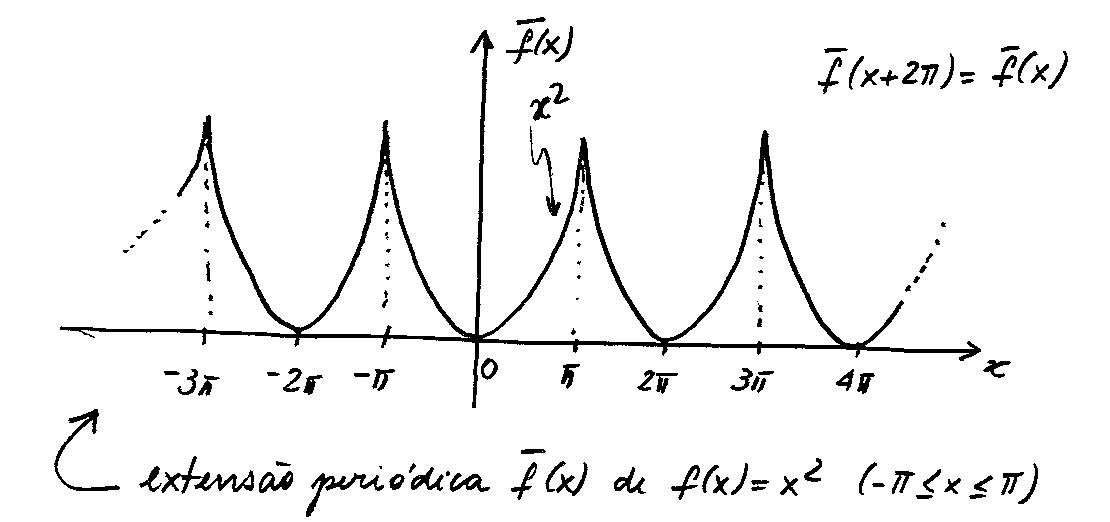
\includegraphics[width=0.8\textwidth]{figuras/serie_fourier_grafico01.jpg}
    \caption{Gr\'{a}fico da s\'{e}rie de Fourier para $f(x) = x^2$.}
    \label{fig:serie_fourier_grafico01}
\end{figure}

\begin{exem}
    Para
    \begin{align*}
        f(x) &= \begin{cases}
            -1, & x < 0, \\
            +1, & x \geq 0.
        \end{cases}
    \end{align*}
    temos que
    \begin{align*}
        a_0 &= \frac{1}{\pi} \int_{-\pi}^\pi f(x) \id{x} \\
        &= \frac{1}{\pi} \left[ -\int_\pi^0 \id{x} + \int_0^\pi \id{x} \right] \\
        &= 0, \\
        a_n &= \frac{1}{\pi} \int_{-\pi}^\pi f(x) \cos\left( n x \right) \id{x} \\
        &= \frac{1}{n} \left[ -\int_{-\pi}^0 \cos\left( n x \right) \id{x} + \int_0^\pi \cos\left( n x \right) \id{x} \right] \\
        &= 0, \\
        b_n &= \frac{1}{\pi} \int_{-\pi}^\pi f(x) \sin\left( n x \right) \id{x} \\
        &= \frac{1}{\pi} \left[ -\int_{-\pi}^0 \sin\left( n x \right) \id{x} + \int_0^\pi \sin\left( n x \right) \id{x} \right] \\
        &= \frac{2}{\pi} \int_0^\pi \sin\left( n x \right) \id{x} \\
        &= \left. \frac{-2 \cos\left( n x \right)}{n \pi} \right|_0^\pi \\
        &= \frac{-2}{n \pi} \left[ (-1)^n - 1 \right] \\
        &= \begin{cases}
            0, & n \text{ \'{e} par}, \\
            4 / \left( n \pi \right), & n \text{ \'{e} \'{i}mpar}.
        \end{cases}
    \end{align*}

    Logo,
    \begin{align*}
        f(x) &= \sum_{n = 1}^\infty b_n \sin\left( n x \right) \\
        &= \sum_{k = 1}^\infty b_{k + 1} \sin\left( (2k + 1) x \right) \\
        &= \sum_{k = 0}^\infty \frac{4}{\left( 2k + 1 \right) \pi} \sin\left( (2k + 1) x \right).
    \end{align*}
\end{exem}

\begin{figure}[!htb]
    \centering
    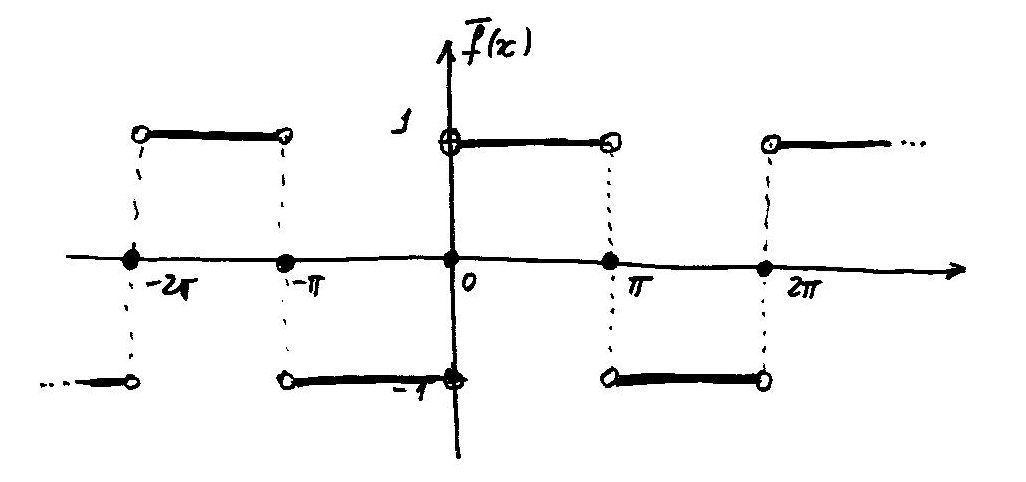
\includegraphics[width=0.8\textwidth]{figuras/serie_fourier_grafico02.jpg}
    % TODO Arrumar o comando \caption abaixo.
    \caption{Gr\'{a}fico da s\'{e}rie de Fourier para }
    \label{fig:serie_fourier_grafico02}
\end{figure}

Pela Figura~\ref{fig:serie_fourier_grafico02} que
\begin{align*}
    \bar{f}(x) &= \begin{cases}
        1, & 0 < x < \pi, \\
        0, & x = 0, \pi, -\pi, \\
        -1, & -\pi < x < 0.
    \end{cases}
\end{align*}
e
\begin{align*}
    \bar{f}(x + 2 \pi) &= \bar{f}(x).
\end{align*}

\begin{obs}
    $\bar{f}(0) \neq f(0)$, o que \'{e} caractyeristico do comportamento da s\'{e}rie de Fourier em uma descontinuidade. Note que
    \begin{align*}
        \bar{f}(0) &= \frac{1}{2} \left[ \lim_{x \to 0^+} f(x) + \lim_{x \to 0^-} f(x) \right]
    \end{align*}
    nesse caso (que se mostrar\'{a} verdade no caso geral!).
\end{obs}

\begin{defi}
    Seja $\mathcal{L}^2[a, b]$ o conjunto das fun\c{c}\~{o}es de quadrado integr\'{a}vel em $a \leq x \leq b$. Dizemos que $f(x)$ e $g(x)$ s\~{a}o ortogonais nesse intervalo se
    \begin{align*}
        \int_a^b f(x) g(x) \id{x} &= 0.
    \end{align*}
\end{defi}

\begin{obs}
    Lembrando que
    \begin{align*}
        0 \leq \left( f - g \right)^2 = f^2 + g^2 - 2 f g,
    \end{align*}
    ou seja,
    \begin{align*}
        2 f g \leq f^2 + g^2,
    \end{align*}
    conclu\'{i}mos que se $f, g \in \mathcal{L}^2[a, b]$, ent\~{a}o existe $\int_a^b f(x) g(x) \id{x}$. Al\'{e}m disso,
    \begin{align*}
        \left( f + g \right)^2 &= f^2 + g^2 + 2 f g \leq 2 \left( f^2 + g^2 \right),
    \end{align*}
    o que garante que $f + g \in \mathcal{L}^2[a, b]$. Como $\mathcal{L}^2[a, b]$ \'{e} um espa\c{c}o vetorial, podemos pesnar nessa integral como o produto escalar $<f, g>$ de $f, g \in \mathcal{L}^2[a, b]$:
    \begin{align*}
        <f, g> = \int_a^b f(x) g(x) \id{x}.
    \end{align*}
\end{obs}

\begin{prop}
    O conjunto $\left\{ 1, \cos\left( n x \right), \sin\left( n x \right) \right\}$ ($n = 1, 2, \ldots$) \'{e} ortogonal em $[-\pi, \pi]$.
\end{prop}
\begin{proof}
    Devemos mostrar que
    \begin{align}
        & \int_{-\pi}^\pi 1 \cos\left( n x \right) \id{x} = \int_{-\pi}^\pi 1 \sin \left( n x \right) \id{x} = 0, \tag{i} \label{eq:serie_fourier_ort01} \\
        & \int_{-\pi}^\pi \cos\left( n x \right) \cos\left( m x \right) \id{x} = \int_{-\pi}^\pi \sin\left( n x \right) \sin\left( m x \right) \id{x} = 0, n \neq m, \tag{ii} \label{eq:serie_fourier_ort02} \\
        & \int_{-\pi}^\pi \cos\left( n x \right) \sin\left( m x \right) \id{x} = 0. \tag{iii} \label{eq:serie_fourier_ort03}
    \end{align}
    As integrais \eqref{eq:serie_fourier_ort01} s\~{a}o triviais. Quanto a \eqref{eq:serie_fourier_ort02} e \eqref{eq:serie_fourier_ort03}, elas s\~{a}o calculadas de forma an\'{a}loga, de modo que faremos explicitamente apenas uma delas. Usando a identidade
    \begin{align*}
        \cos\left( n x \right) \cos\left( m x \right) &= \frac{1}{2} \cos\left( (n - m) x \right) + \frac{1}{2} \cos\left( (n + m) x \right)
    \end{align*}
    segue, para $n \neq m$, que
    \begin{align*}
        \int_{-\pi}^\pi \cos\left( n x \right) \cos\left( m x \right) \id{x} = \frac{1}{2} \left. \frac{\sin\left( (n - m) x \right)}{n - m} \right|_{-\pi}^\pi + \frac{1}{2} \left. \frac{\sin\left( (n + m) x \right)}{n - m} \right|_{-\pi}^\pi = 0
    \end{align*}
    pois $\sin\left( k \pi \right) = 0$ para $k$ inteiro.

    N\~{a}o custa chamar a aten\c{c}\~{a}o para o fato que \eqref{eq:serie_fourier_ort03} vale para quaisquer $n$ e $m$, enquanto \eqref{eq:serie_fourier_ort02} vale para $n \neq m$. Quando $n = m$, para \eqref{eq:serie_fourier_ort02} temos
    \begin{align*}
        \int_{-\pi}^\pi \cos^2\left( n x \right) \id{x} = \int_{-\pi}^\pi \sin^2\left( n x \right) \id{x} = \pi.
    \end{align*}
\end{proof}

\begin{teo}
    Se uma s\'{e}rie trigonom\'{e}trica converge uniformemente para a fun\c{c}\~{a}o $f(x)$ em $-\pi \leq x \leq \pi$, ent\~{a}o ela \'{e} a s\'{e}rie de Fourier de $f(x)$.
\end{teo}
\begin{proof}
    Se
    \begin{align*}
        f(x) = \frac{A_0}{2} + \sum_{n = 1}^\infty \left( A_n \cos\left( n x \right) + B_n \sin\left( n x \right) \right)
    \end{align*}
    converge uniformentente, o mesmo acontecer\'{a} com a s\'{e}rie multiplicada por $\cos\left( m x \right)$ ou $\sin\left( m x \right)$. Como uma s\'{e}rie uniformemente convergente pode ser integrada termo a termo, temos, por exemplo
    \begin{align*}
        \begin{split}
            \int_{-\pi}^\pi f(x) \cos\left( m x \right) \id{x} &= \frac{A_0}{2} \underbrace{\int_{-\pi}^\pi \cos\left( m x \right) \id{x}}_{= 0} \\
            &\quad {}+ \sum_{n = 1}^\infty \left( A_n \underbrace{\int_{-\pi}^\pi \cos\left( n x \right) \cos\left( m x \right) \id{x}}_{= 0 (n \neq m)} + B_n \underbrace{\int_{-\pi}^\pi \sin\left( n x \right) \cos\left( m x \right) \id{x}}_{= 0} \right)
        \end{split}
    \end{align*}
    onde usamos a proposi\c{c}\~{a}o anterior, de modo que
    \begin{align*}
        \int_{-\pi}^\pi f(x) \cos\left( m x \right) \id{x} &= A_m \int_{-\pi}^\pi \cos^2\left( m x \right) \id{x} = \pi A_m,
    \end{align*}
    ou seja, $A_m$ \'{e} um coeficiente de Fourier. Procedendo de forma an\'{a}logo, veremos que o mesmo acontece com $A_0$ e $B_m$, de modo que se trat a de uma s\'{e}rie de Fourier.
\end{proof}

\section{Mudan\c{c}a de intervalo}
Vamos agora, ao inv\'{e}s de $T = 2 \pi$, considerar um per\'{i}odo $T = 2 L$. Para isso, na s\'{e}rie de Fourier
\begin{align*}
    f(x') = \frac{a_0}{2} + \sum_{n = 1}^\infty \left( a_n \cos\left( n x' \right) + b_n \sin\left( n x' \right) \right),
\end{align*}
vamos fazer a mudan\c{c}a de vari\'{a}vel
\begin{align*}
    x' = \frac{\pi}{L} x.
\end{align*}
Assim, para $f(x') = f(\pi x / L) = f(x)$, temos
\begin{align*}
    F(x) &= \frac{a_0}{2} + \sum_{n = 1}^\infty \left( a_n \cos\left( \frac{n \pi x}{L} \right) + b_n \sin\left( \frac{n \pi x}{L} \right) \right),
\end{align*}
com
\begin{align*}
    a_n &= \frac{1}{\pi} \int_{-\pi}^\pi f(x') \cos\left( n x' \right) \id{x'} = \frac{1}{\pi} \int_{-L}^L \frac{\pi}{L} f\left( \frac{\pi}{L} x \right) \cos\left( \frac{n \pi x}{L} \right) \id{x},
\end{align*}
ou seja,
\begin{align*}
    a_n &= \frac{1}{L} \int_{-L}^L F(x) \cos\left( \frac{n \pi x}{L} \right) \id{x}, & n = 1, 2, \ldots
\end{align*}
e da mesma forma
\begin{align*}
    b)n &= \frac{1}{L} \int_{-L}^L F(x) \sin\left( \frac{n \pi x}{L} \right) \id{x} & n = 1, 2, \ldots
\end{align*}

\begin{exem}
    Para $f(x) = x^2, - 2 \pi \leq x \leq 2 \pi$ temos, usando $L = 2 \pi$ (portanto per\'{i}odo $T = 4\pi$), encontramos que
    \begin{align*}
        x^2 = \frac{4 \pi^2}{3} + \sum_{n = 1}^\infty \frac{16 (-1)^n}{n^2} \cos\left( \frac{n x}{2} \right).
    \end{align*}
\end{exem}

\section{Forma complexa}
Temos que $\exp(i x) = \cos(x) + i \sin(x)$ e portanto
\begin{align*}
    \cos\left( \frac{n \pi x}{L} \right) &= \frac{1}{2} \left( \exp\left( i \frac{n \pi x}{L} \right) + \exp\left( -i \frac{n \pi x}{L} \right) \right), \\
    \sin\left( \frac{n \pi x}{L} \right) &= \frac{1}{2 i} \left( \exp\left( i \frac{n \pi x}{L} \right) - \exp\left( -i \frac{n \pi x}{L} \right) \right).
\end{align*}
Logo,
\begin{align*}
    \begin{split}
        f(x) &= \frac{a_0}{2} + \sum_{n = 1}^\infty \left[ \frac{a_n}{2} \exp\left( i \frac{n \pi x}{L} \right) + \frac{a_n}{2} \exp\left( -i \frac{n \pi x}{L} \right) \right.\\ &\quad \left. {}- \frac{b_n i}{2} \exp\left( i \frac{n \pi x}{L} \right) + \frac{b_n i}{2} \exp\left( -i \frac{n \pi x}{L} \right) \right]
    \end{split} \\
    &= \frac{a_0}{2} + \sum_{n = 1}^\infty \underbrace{\left( \frac{a_n - i b_n}{2} \right)}_{c_n} \exp\left( i \frac{n \pi x}{L} \right) + \sum_{n = 1}^\infty \underbrace{\left( \frac{a_n + i b_n}{2} \right)}_{c_n^*} \exp\left( -i \frac{n \pi x}{L} \right)
\end{align*}

\begin{defi}
    Temos que $c_{- n} = c_n^*$, portanto
    \begin{align*}
        c_n &= \begin{cases}
            \left( 1/2 \right) \left( a_n - i b_n \right), & n = 1, 2, \ldots \\
            \left( 1/2 \right) \left( a_n + i b_n \right), & n = -1, -2, \ldots \\
            \left( 1/2 \right) a_0, & n = 0.
        \end{cases}
    \end{align*}
    Logo,
    \begin{align*}
        f(x) &= c_0 + \sum_{n = 1}^\infty c_n \exp\left( i (n \pi x) / L \right) + \sum_{n = -1}^{-\infty} \underbrace{\left( 1/2) \right) \left( a_{-n} + i b_{-n} \right)}_{c_n} \exp\left( i (n \pi x) / L \right) \\
        &= \sum_{n = -\infty}^\infty c_n \exp\left( i (n \pi x) / L \right).
    \end{align*}
\end{defi}

\begin{obs}
    Note que
    \begin{align*}
        f^*(x) &= \sum_{n = -\infty}^\infty c_n^* \exp\left( -i n \pi x / L \right) \\
        &= \sum_{n = -\infty}^`9 c_{-n}^* \exp\left( i n \pi x / L \right) \\
        &= \sum_{n = -\infty}^\infty c_n \exp\left( i n \pi x / L \right) \\
        &= f(x).
    \end{align*}
\end{obs}

E $c_n$ \'{e} obtido por
\begin{align*}
    \int_{-L}^L \exp\left( -i m \pi x / L \right) \exp\left( i n \pi x / L \right) \id{x} &= \int_{-L}^L \exp\left( i (n - m) \pi x / L \right) \id{x} \\
    &= \begin{cases}
        \int_{-L}^L \id{x} = 2 L, & n = m, \\
        \left. \exp\left( i (n - m) \pi x / L \right) \left( i (n - m) \pi / L \right)^{-1} \right|_{-L}^L = 0
    \end{cases} \\
    &= 2 L \delta_{mn}.
\end{align*}
Com isso
\begin{align*}
    \int_{-L}^L f(x) \exp\left( -i m \pi x / L \right) \id{x} &= \sum_{n = -\infty}^\infty c_n \int_{-L}^L \exp\left( i n \pi x / L \right) \exp\left( -i m \pi x / L \right) \id{x} \\
    &= 2 L \sum_{n = \infty}^\infty c_n \delta_{mn} \\
    &= 2 L c_m.
\end{align*}
Logo,
\begin{align*}
    c_n &= \frac{1}{2L} \int_{-L}^L f(x) \exp\left( -i n \pi x / L \right) \id{x}.
\end{align*}

\begin{exem}
    Seja $f(x)$ dado por
    \begin{align*}
        f(x) &= \begin{cases}
            1 / 2a, & |x| \leq a, \\
            0, & |x| > a,
        \end{cases}
    \end{align*}
    onde $a < L$. Logo, temos
    \begin{align*}
        c_n &= \frac{1}{2L} \int_{-L}^L f(x) \exp\left( -i n \pi x / L \right) \id{x} \\
        &= \frac{1}{2L} \int_{-a}^a \frac{1}{2a} \exp\left( -i n \pi x / L \right) \\
        &= \frac{1}{2L} \frac{1}{2a} \left. \frac{\exp\left( -i n \pi x / L \right)}{- i n \pi / L} \right|_{-a}^a \\
        &= \frac{1}{2 (2a) (-i n \pi)} \left( \exp\left( -i n \pi a / L \right) - \exp\left( i n \pi a / L \right) \right) \\
        &= \frac{1}{2 a n \pi} \left( \frac{\exp\left( i n \pi a / L \right) - \exp\left( -i n \pi a / L \right)}{2 i} \right) \\
        &= \sin\left( n \pi a / L \right) \left( 2 n \pi a \right)^{-1}.
    \end{align*}
    E portanto,
    \begin{align*}
        f(x) = \sum_{n = -\infty}^\infty \frac{\sin\left( n \pi a / L \right)}{2 n \pi a} \exp\left( i n \pi a / L \right).
    \end{align*}
    Tamb\'{e}m \'{e} poss\'{i}vel
    \begin{align*}
        f(x) &= \frac{1}{2 L} + \sum_{n = 1}^\infty \frac{\sin\left( n \pi a / L \right)}{2 n \pi a} \exp\left( i n \pi a / L \right) + \sum_{n = 1}^\infty \frac{\sin\left( (-n) \pi a / L \right)}{2 (-n) \pi a} \exp\left( i (-n) \pi a / L \right) \\
        &= \frac{1}{2L} + \sum_{n = 1}^\infty \frac{\sin\left( n \pi a / L \right)}{2 n \pi a} \left( \exp\left( i n \pi a / L \right) + \exp\left( -i n \pi a / L \right) \right) \\
        &= \frac{1}{2L} + \sum_{n = 1}^\infty \frac{\sin\left( n \pi a / L \right)}{n \pi a} \cos\left( n \pi a / L \right).
    \end{align*}
\end{exem}

\section{Propriedades de Paridade: S\'{e}ries em Seno e Cosseno}
Temos, por defini\c{c}\~{a}o que
\begin{align*}
    f(-x) &= \begin{cases}
        f(x) \Rightarrow f \text{ \'{e} par}, \\
        -f(x) \Rightarrow f \text{ \'{e} \'{i}mpar}.
    \end{cases}
\end{align*}
Debotando uma fun\c{c}\~{a}o par por $f_+(x)$ e uma fun\c{c}\~{a}o \'{i}mpar por $f_-(x)$ temos
\begin{align*}
    f_\pm(-x) &= \pm f_\pm(x).
\end{align*}

\begin{prop}
    Temos que
    \begin{align*}
        \int_{-L}^L f(x) \id{x} &= \begin{cases}
            2 \int_0^L f(x) \id{x}, & f \text{ \'{e} par}, \\
            0, & f \text{ \'{e} \'{i}mpar}.
        \end{cases}
    \end{align*}
\end{prop}
\begin{proof}
    Temos que
    \begin{align*}
        \int_{-L}^L f_\pm(x) \id{x} &= \int_{-L}^0 f_\pm(x) \id{x} + \int_0^L f_\pm(x) \id{x} \\
        &= -\int_{-L}^0 f_\pm(-x) \id{x} + \int_0^L f_\pm(x) \id{x} \\
        &= \int_0^L f_\pm(-x) \id{x} + \int_0^L f_\pm(x) \id{x} \\
        &= \pm \int_0^L f_\pm(x) \id{x} + \int_0^L f_\pm(x) \id{x} \\
        &= \begin{cases}
            2 \int_0^L f_\pm(x) \id{x}, & \text{para } f_+, \\
            0, & \text{para } f_-.
        \end{cases}
    \end{align*}
\end{proof}

Por outro lado, \'{e} f\'{a}cil verificar as informa\c{c}\~{o}es da tabela abaixo.
\begin{table}[htb]
    \centering
    \begin{tabular}{|c|c|c|}
        \hline
        $f(x)$ & $g(x)$ & $f(x) g(x)$ \\ \hline
        par & par & par \\ \hline
        \'{i}mpar & par & \'{i}mpar \\ \hline
        \'{i}mpar & \'{i}mpar & par \\ \hline
    \end{tabular}
\end{table}

Logo, da proposi\c{c}\~{a}o:
\begin{align*}
    a_n &= \frac{1}{L} \int_{-L}^L f(x) \cos\left( n \pi x / L \right) \id{x} = 0 \\
    \intertext{se $f(x)$ \'{e} \'{i}mpar e}
    b_n &= \frac{1}{L} \int_{-L}^L f(x) \sin\left( n \pi x / L \right) \id{x} = 0
\end{align*}
se $f(x)$ \'{e} par.

Logo:
\begin{enumerate}
    \item se $f(x) = f_+(x)$ \'{e} par:
        \begin{align*}
            f_+(x) &= \frac{a_0}{2} + \sum_{n = 1}^\infty a_n \cos\left( n \pi x / L \right), \\
            a_n &= \frac{2}{L} \int_0^L f(x) \cos\left( n \pi x / L \right) \id{x}
        \end{align*}
        que \'{e} a S\'{e}rie de Fourier em cossenos.
    \item Se $f(x) = f_-(x)$ \'{e} \'{i}mpar:
        \begin{align*}
            f_-(x) &= \sum_{n = 1}^\infty n_n \sin\left( n \pi x / L \right), \\
            b_n &= \frac{2}{L} \int_0^L f(x) \sin\left( n \pi x / L \right) \id{x}
        \end{align*}
        que \'{e} a S\'{e}rie de Fourier em senos.
\end{enumerate}

\begin{exem}
    Considere $f(x) = x / \left( 2 L \right) + 1 / 2$ cujo gr\'{a}fico \'{e} ilustrado abaixo.
    % TODO Inserir gr\'{a}fico de $f(x)$.
    \begin{enumerate}
        \item S\'{e}rie de Fourier:
            \begin{align*}
                a_0 &= \frac{1}{L} \int_{-L}^L \left( \frac{x}{2 L} + \frac{1}{2} \right) \id{x} \\
                &= \left. \frac{1}{L} \left( \frac{x^2}{4 L} + \frac{x}{2} \right) \right|_{-L}^L \\
                &= 1, \\
                a_n &= \frac{1}{L} \int_{-L}^L \cos\left( n \pi x / L \right) \left( \frac{x}{2 L} + \frac{1}{2} \right) \id{x} \\
                &= \frac{1}{2 L^2} \int_{-L}^L x \cos\left( n \pi x / L \right) \id{x} + \frac{1}{2L} \int_{-L}^L \cos\left( n \pi x / L \right) \id{x} \\
                &= 0,
                b_n &= \frac{1}{L} \int_{-L}^L \sin\left( n \pi x / L \right) \left( \frac{x}{2L} + \frac{1}{2} \right) \id{x} \\
                &= \frac{1}{2L^2} \int_{-L}^L x \sin\left( n \pi x / L \right) \id{x} + \frac{1}{2L} \int_{-L}^L \sin\left( n \pi x / L \right) \id{x} \\
                &= \frac{1}{2L^2} \left[ \left. \frac{-x \cos\left( n \pi x / L \right)}{n \pi / L} \right|_{-L}^L + \frac{1}{n \pi / L} \int_{-L}^L \cos\left( n \pi x / L \right) \right] \\
                &= \frac{1}{2L^2} \frac{\left( -2L^2 \right) \left( -1 \right)^n}{n \pi} \\
                &= \frac{(-1)^{n + 1}}{n \pi}.
            \end{align*}
            Logo,
            \begin{align*}
                F(x) &= \frac{1}{2} + \sum_{n = 1}^\infty \frac{(-1)^{n + 1}}{n \pi} \sin\left( n \pi x / L \right).
            \end{align*}
            % TODO Incluir gr\'{a}fico.

        \item S\'{e}rie de Fourier em senos:
            \begin{align*}
                b_n &= \frac{2}{L} \int_0^L \sin\left( n \pi x / L \right) \left( \frac{x}{2} + \frac{1}{2} \right) \id{x} \\
                &= \frac{1}{L^2} \int_0^L x \sin\left( n \pi x / L \right) \id{x} + \frac{1}{L} \int_0^L \sin\left( n \pi x / L \right) \id{x} \\
                &= \frac{1}{L^2} \left[ \left. \frac{- x \cos\left( n \pi x / L \right)}{n \pi / L} \right|_0^L + \frac{L}{n \pi} \int_0^L \cos\left( n \pi x / L \right) \id{x} \right] + \frac{1}{L} \left. \frac{- \cos\left( n \pi x / L \right)}{n \pi / L} \right|_0^L \\
                &= \frac{-1}{n \pi} \cos\left( n \pi \right) - \frac{1}{n \pi} \cos\left( n \pi \right) + \frac{1}{n \pi} \\
                &= \frac{1 - 2 (-1)^n}{n \pi}.
            \end{align*}
            Logo,
            \begin{align*}
                F_-(x) &= \sum_{n = 1}^\infty \left( \frac{1 - 2 (-1)^n}{n \pi} \right) \sin\left( n \pi x / L \right).
            \end{align*}
            % TODO Incluir gr\'{a}fico.

        \item S\'{e}rie de Fourier em cossenos:
            \begin{align*}
                a_0 &= \frac{2}{L} \int_0^L \left( \frac{x}{2L} + \frac{1}{2} \right) \id{x} \\
                &= \frac{2}{L} \left. \left( \frac{x^2}{4 L} + \frac{x}{2} \right) \right|_0^L \\
                &= \frac{3}{2}. \\
                a_n &= \frac{2}{L} \int_0^L \left( \frac{x}{2L} + \frac{1}{2} \right) \cos\left( n \pi x / L \right) \\
                &= \frac{1}{L^2} \int_0^L x \cos\left( n \pi x / L \right) \id{x} + \frac{1}{L} \int_0^L \cos\left( n \pi x / L \right) \id{x} \\
                &= \frac{1}{L^2} \left[ \left. \frac{x \sin\left( n \pi x / L \right)}{n \pi / L} \right|_0^L - \frac{L}{n \pi} \int_0^L \sin\left( n \pi x / L \right) \id{x} \right] + \frac{1}{L} \frac{1}{n \pi / L} \left. \sin\left( n \pi x / L \right) \right|_0^L \\
                &= \frac{1}{L n \pi} \left. \frac{\cos\left( n \pi x / L \right)}{n \pi / L} \right|_0^L \\
                &= \frac{1}{n^2 \pi^2} \left[ (-1)^n - 1 \right].
            \end{align*}
            Logo,
            \begin{align*}
                F_+(x) &= \frac{3}{4} + \sum_{n = 1}^\infty \frac{\left[ (-1)^n - 1 \right]}{n^2 \pi^2} \cos\left( n \pi x / L \right).
            \end{align*}
            % TODO Incluir gr\'{a}fico.
    \end{enumerate}
\end{exem}

\section{Teorema de Fourier}
Para facilitar a nota\c{c}\~{a}o, vamos tomar $L = \pi$. Ent\~{a}o
\begin{align*}
    f(x) &= \frac{a_0}{2} + \sum_{n = 1}^\infty \left( a_n \cos\left( n x \right) + b_n \sin\left( n x \right) \right) \\
    \begin{split}
        &= \frac{1}{2} \left[ \frac{1}{\pi} \int_{-\pi}^\pi f(\xi) \id{\xi} \right] \\ &\quad {}+ \sum_{n = 1}^\infty \left[ \left( \frac{1}{\pi} \int_{-\pi}^\pi f(\xi) \cos\left( n \xi \right) \id{\xi} \right) \cos\left( n x \right) + \left( \frac{1}{\pi} \int_{-\pi}^\pi f(\xi) \sin\left( n \xi \right) \id{\xi} \right) \sin\left( n x \right) \right]
    \end{split} \\
    &= \frac{1}{2\pi} \int_{-\pi}^\pi f(\xi) \id{\xi} + \frac{1}{\pi} \sum_{n = 1}^\infty \int_{-\pi}^\pi f(\xi) \left[ \cos\left( n \xi \right) \cos\left( n x \right) + \sin\left( n \xi \right) \sin\left( n x \right) \right] \id{\xi}.
\end{align*}
Portanto,
\begin{align}
    f(x) &= \frac{1}{2\pi} \int_{-\pi}^\pi f(\xi) \id{\xi} + \frac{1}{\pi} \sum_{n = 1}^\infty \int_{-\pi}^\pi f(\xi) \cos\left( n (\xi - x) \right) \id{\xi}.
    \label{eq:serie_fourier}
\end{align}

\begin{teo}[Fourier]
    Seja $f(x)$ uma fun\c{c}\~{a}o cont\'{i}nua por partes e com derivadas laterais no intervalo $(-\pi, \pi)$ e peri\'{o}dica com per\'{i}odo $2\pi$. Ent\~{a}o sua s\'{e}rie de Fourier, \eqref{eq:serie_fourier}, converge para o valor
    \begin{align*}
        \frac{1}{2} \left[ f(x + 0) + f(x - 0) \right]
    \end{align*}
    em $-\infty < x < \infty$.
\end{teo}

Antes de provarmos o teorema de Fourier precisamos explicitar o que entendemos por derivadas laterais e provar alguns lemas auxiliares.

\subsection{Derivadas Laterais}
% TODO Terminar de incluir arquivo M2S12-2.pdf. Interrompido na p\'{a}gina 10.

% TODO Incluir arquivo M2S12-3.pdf

\section{Converg\^{e}ncia na M\'{e}dia}
Da express\~{a}o para o produto escalar em $\mathcal{L}^2(a, b)$ definimos uma norma atrav\'{e}s de
\begin{align*}
    \| f \|^2 &= <f, f> = \int_a^b \left[ f(x) \right]^2 \id{x}.
\end{align*}

Com isso, dados as fun\c{c}\~{o}es $f, g \in \mathcal{L}^2(a, b)$, definimos o desvio total quadr\'{a}tico dessas fun\c{c}\~{o}es como
\begin{align*}
    \Delta &= \| f - g \|^2 = \int_a^b \left[ f(x) - g(x) \right]^2 \id{x}.
\end{align*}

\begin{teo}
    Seja o polin\^{o}mio trigonom\'{e}trico
    \begin{align*}
        \phi_N(x) &= \frac{A_0}{2} + \sum_{n = 1}^N \left( A_n \cos\left( n x \right) + B_n \sin\left( n x \right) \right),
    \end{align*}
    onde $A_0$, $A_n$ e $B_n$ s\~{a}o indeterminados e $f(x)$ \'{e} uma fun\c{c}\~{a}o cont\'{i}nua por partes em $[-\pi, \pi]$. Ent\~{a}o o desvio total quadr\'{a}tico $\Delta_N = \| f - \phi_N \|^2$ \'{e} minimizado quando os coeficientes $A_0$, $A_n$ e $B_n$ forem iguais aos coeficientes de Fourier de $f(x)$.
\end{teo}
\begin{proof}
    Temos que
    \begin{align*}
        \Delta_n &= \int_{-\pi}^\pi \left[ f(x) - \phi_N(x) \right]^2 \id{x} \\
        &= \int_{-\pi}^\pi \left[ f(x) - \frac{A_0}{2} - \sum_{n = 1}^N \left( A_n \cos\left( n x \right) + B_n \sin\left( n x \right) \right) \right]^2 \id{x} \\
        \begin{split}
            &= \int_{-\pi}^\pi \left[ f(x) \right]^2 \id{x} + \int_{-\pi}^\pi \left( \frac{A_0}{2}^2 \right) \id{x} + \int_{-\pi}^\pi \sum_{n = 1}^N \sum_{m = 1}^N A_n A_m \cos\left( n x \right) \cos\left( m x \right) \id{x} \\
            &\quad {}+ \int_{-\pi}^\pi \sum_{n = 1}^N \sum_{m = 1}^N B_n B_m \sin\left( n x \right) \sin\left( m x \right) \id{x} - 2 \int_{-\pi}^\pi f(x) \frac{A_0}{2} \id{x} - 2 \int_{-\pi}^\pi f(x) \sum_{n = 1}^N \cos\left( n x \right) \id{x} \\
            &\quad {}- 2 \int_{-\pi}^\pi f(x) \sum_{n = 1}^N B_n \sin\left( n x \right) \id{x} + 2 \int_{-\pi}^\pi \frac{A_0}{2} \cos\left( n x \right) \id{x} + 2 \int_{-\pi}^\pi \frac{A_0}{2} \sum){n = 1}^N B_n \sin\left( n x \right) \id{x} \\
            &\quad {}+ 2 \int_{-\pi}^\pi \sum_{n = 1}^N \sum_{m = 1}^N A_n B_n \cos\left( n x \right) \sin\left( m x \right) \id{x}
        \end{split} \\
        \begin{split}
            &= \int_{-\pi}^\pi \left[ f(x) \right]^2 \id{x} + \frac{A_0^2}{4} 2 \pi + \sum_{n = 1}^N \sum_{m = 1}^N A_n A_m \underbrace{\int_{-\pi}^\pi \cos\left( n x \right) \cos\left( m x \right) \id{x}}_{\pi \delta_{nm}} \\
            &\quad {}+ \sum_{n = 1}^N \sum_{m = 1}^N B_n B_m \underbrace{\int_{-\pi}^\pi \sin\left( n x \right) \sin\left( m x \right) \id{x}}_{\pi \delta_{nm}} - A_0 \int_{-\pi}^\pi f(x) \id{x} - 2 \sum_{n = 1}^N A_n \int_{-\pi}^\pi f(x) \cos\left( n x \right) \id{x} \\
            &\quad {}- 2 \sum_{n = 1}^N B_n \int_{-\pi}^\pi f(x) \sin\left( n x \right) \id{x} + A_0 \sum_{n = 1}^N A_n \underbrace{\int_{-\pi}^\pi \cos\left( n x \right) \id{x}}_{=0} + A_0 \sum_{n = 1}^N B_n \underbrace{\int_{-\pi}^\pi \sin\left( n x \right) \id{x}}_{=0} \\
            &\quad {}+ 2 \sum_{n = 1}^N \sum_{m = 1}^N A_n B_m \underbrace{\int_{-\pi}^\pi \cos\left( n x \right) \sin\left( m x \right) \id{x}}_{=0}
        \end{split}
    \end{align*}
    Portanto,
    \begin{align*}
        \begin{split}
            \delta_N &= \int_{-\pi}^\pi \left[ f(x) \right]^2 \id{x} + \frac{\pi}{2} A_0^2 + \sum_{n = 1}^N \pi A_n^2 + \sum_{n = 1}^N \pi B_n^2 \\
            &\quad {}- A_0 \int_{-\pi}^\pi f(x) \id{x} - 2 \sum_{n = 1}^N A_n \int_{-\pi}^\pi f(x) \cos\left( n x \right) \id{x} - 2 \sum_{n = 1}^N B_n \int_{-\pi}^\pi f(x) \sin\left( n x \right) \id{x}
        \end{split}
    \end{align*}
    Exigindo agora que
    \begin{align*}
        \devp{\Delta_N}{A_0} &= \devp{\Delta_N}{A_n} = \devp{\Delta_N}{B_n} = 0
    \end{align*}
    para $n = 1, \ldots, N$ temos que
    \begin{align*}
        & \devp{\Delta_N}{A_0} = \pi A_0 - \int_{-\pi}^\pi f(x) \id{x} = 0 \Rightarrow A_0 = \frac{1}{\pi} \int_{-\pi}^\pi f(x) \id{x} = a_0, \\
        & \devp{\Delta_N}{A_n} = 2 \pi A_n - 2 \int_{-\pi}^\pi f(x) \cos\left( n x \right) \id{x} = 0 \Rightarrow A_n = \frac{1}{\pi} \int_{-\pi}^\pi f(x) \cos\left( n x \right) \id{x} = a_n, \\
        & \devp{\Delta_N}{B_n} = 2 \pi B_n - 2 \int_{-\pi} \pi f(x) \sin\left( n x \right) \id{x} = 0 \Rightarrow B_n = \frac{1}{\pi} \int_{-\pi}^\pi f(x) \sin\left( n x \right) \id{x} = b_n.
    \end{align*}
    Al\'{e}m disso, \'{e} f\'{a}cil ver que o extremo em quest\~{a}o \'{e} um m\'{i}nimo.
\end{proof}

Com isso, temos que $\Delta_n^{\min}$ \'{e} dado por
\begin{align*}
    \begin{split}
        \Delta_N^{\min} &= \int_{-\pi}^\pi \left[ f(x) \right]^2 \id{x} + \frac{\pi}{2} a_0^2 + \sum_{n = 1}^N \pi a_n^2 + \sum_{n = 1}^N \pi b_k^2 \\
        &\quad {}- a_0 \left( \pi a_0 \right) - 2 \sum_{n = 1}^N a_n \left( \pi a_n \right) - 2 \sum_{n = 1}^N b_n \left( \pi b_n \right)
    \end{split}
\end{align*}
e portanto
\begin{align*}
    \Delta_N^{\min} &= \int_{-\pi}^\pi \left[ f(x) \right]^2 \id{x} - \pi \left[ \frac{a_0^2}{2} + \sum_{n = 1}^N \left( a_n^2 + b_n^2 \right) \right].
\end{align*}
Al\'{e}m disso, como $\Delta_N \geq 0$, temos que
\begin{align*}
    \frac{a_0^2}{2} + \sum_{n = 1}^N \left( a_n^2 + b_n^2 \right) \leq \frac{1}{\pi} \int_{-\pi}^\pi \left[ f(x) \right]^2 \id{x}.
\end{align*}

\begin{prop}
    Os coeficientes de Fourier satisfazem a chamada desigualdade de Bessel:
    \begin{align*}
        \frac{a_0^2}{2} + \sum_{n = 1}^\infty \left( a_n^2 + b_n^2 \right) \leq \frac{1}{\pi} \int_{-\pi}^\pi \left[ f(x) \right]^2 \id{x}.
    \end{align*}
\end{prop}
\begin{proof}
    Seja a sequ\^{e}ncia $\left\{ \Delta_N \right\}$, onde
    \begin{align*}
        \Delta_N = \frac{a_0^2}{2} + \sum_{n = 1}^N \left( a_n^2 + b_n^2 \right).
    \end{align*}
    Como consequ\^{e}ncia de $\Delta_n \geq 0$, temos acima que essa sequ\^{e}ncia \'{e} limitada. Al\'{e}m disso, ela \'{e} evidentemente mon\'{o}tona. Como uma sequencia mon\'{o}tona e limitada \'{e} convergente, segue que existe $\lim_{N \to \infty} \Delta_N$ satisfazendo essa desigualdade.
\end{proof}
% TODO Terminar de incluir arquivo M2S12-4.pdf. Interrompido na p\'{a}gina 5.

% TODO Incluir arquivo M2S12-5.pdf
% TODO Incluir arquivo M2S12-6.pdf
% TODO Incluir arquivo M2S12-7.pdf
